\documentclass[t]{beamer}

%\documentclass[handout, t]{beamer}
\setbeamertemplate{navigation symbols}{}
\usepackage{pstricks}
\usepackage{mathtools}
\usepackage{amsfonts}
\usepackage{mathrsfs}
\usepackage{amsmath}
\setbeamertemplate{navigation symbols}{}
\usepackage{bm}
\usepackage[UTF8]{ctex}
\usetheme{AnnArbor}
\usefonttheme{serif}
\useinnertheme{rounded}
%\usecolortheme{crane}
\setbeamertemplate{blocks}[rounded][shadow=true]

\newcommand{\dif}{{\;\rm d}}
\usepackage{graphicx}
\usepackage{pgf}
\usepackage{tikz}
\usetikzlibrary{arrows, decorations.pathmorphing, backgrounds, positioning, fit, petri, automata}
\tikzset{>=stealth}


\setmainfont{Times New Roman}
\setCJKmainfont{Microsoft YaHei}


\hypersetup{pdfpagemode=FullScreen}
\renewcommand{\Pr}{\mathbb{P}}
\usepackage{blkarray}


\setbeamercolor{block title}{bg=red!10!white}
\setbeamercolor{block body}{bg=gray!10!white}

\usepackage{multicol}
\newcommand{\E}{\mathbb{E}}
\newcommand{\EP}{\mathbb{E}^{\mathbb{P}}}
\newcommand{\EQ}{\mathbb{E}^{\mathbb{Q}}}
\newcommand{\Var}{{\rm Var}}
\newcommand{\Cov}{{\rm Cov}}

\usepackage{listings}


\lstset{
  language=SQL, % 设置语言
  basicstyle=\ttfamily, % 设置字体族
  breaklines=true, % 自动换行
  keywordstyle=\bfseries\color{blue}, % 设置关键字
  ndkeywordstyle=\bfseries\color{blue}, % 设置关键字
  classoffset=0,
  emph=[0]{self, plt, pd, np, print, sm, sns, None, True, False}, % 指定强调词,如果有多个,用逗号隔开
  emphstyle=\bfseries\color{magenta!90!black}, % 强调词样式设置
  classoffset=1,
  moreemph=[1]{import, plot, text, title, show, scatter, as, figure, xlabel, ylabel, fit, mean, merge}, % 设置更多的关键字,用逗号分隔
  emphstyle=\bfseries\color{blue}, % 强调词样式设置
  classoffset=0,
  commentstyle=\itshape\color{gray}, % 设置注释样式,斜体,浅灰色
  stringstyle=\bfseries\color{green!50!black}, % 设置字符串样式
  columns=flexible,
  numberstyle=\footnotesize, % 缩小行号
}

\begin{document}
\fontsize{11}{18}\selectfont


\CTEXindent



  \title{第二章~~金融数据库搭建及使用}
\author{方杰、李烜}
\date{福建江夏学院金融学院}
  \begin{frame}
    \maketitle
  \end{frame}

\begin{frame}{本章内容}
  \begin{multicols}{2}
    \tableofcontents
  \end{multicols}
\end{frame}

\section{数据库基础知识}
\subsection{数据库的概念及分类}
\begin{frame}
    \frametitle{数据库的概念}
\begin{itemize}
  \item 数据库是“按照数据结构来组织、存储和管理数据的仓库”,是一个长期存储 在计算机内的、有组织的、可共享的、统一管理的大量数据的集合。
  \item 从狭义的方面来讲,数据库是用于存储数据的地方,相当于一个电子化的文件柜。
  一个数据库可能包含多个表或者文件,一个数据库系统中通常包含多个数据库。
  \item 从广义的方面理解,数据库不仅是一个存储数据的容器,还是一个按数 据结构来存储和管理数据的计算机软件系统。
\end{itemize}
    

\end{frame}

\begin{frame}
    \frametitle{数据库的分类}
\begin{itemize}
  \item 层次式数据库
  \item 网络式数据库
  \item {\color{red}关系型数据库}
  \item 非关系型数据库
\end{itemize}
    

\end{frame}

\subsection{关系型数据库}

\begin{frame}
    \frametitle{关系型数据库}
    关系型数据库存指采用了关系模型来组织数据,由二维表及其之间的联系组成的一个数据组织。一个关系 型数据库中可以包含一个或多个表格,表格间如存在一定的关系,可通过联结(join)语句对表建立关系
\begin{multicols}{2}
\begin{itemize}
  \item 优点
  \begin{itemize}
    \item 易理解\\~\\ \item 使用方便\\~\\ \item  易维护
  \end{itemize}
  \item 缺点
  \begin{itemize}
    \item 硬盘I/O压力大
    \item  不适用于非结构化数据 \item  横向扩展性差
    \item  性能欠佳
  \end{itemize}
\end{itemize}
\end{multicols}

\end{frame}

\begin{frame}
    \frametitle{主流的关系型数据库}
\begin{itemize}
  \item Oracle:甲骨文公司出品 的一款以分布式数据库为核心的关系数据库管理系统。
  \item MySQL:由瑞典MySQL AB 公司开发,属于 Oracle 旗下产品。MySQL
   是最流行的关系型数据库管理系统之一。
   \item SQL Server:微软公司推出的关系型数据库管 理系统,适合大容量的数据存储,可扩展性强、相关 软件集成度高,并且操作简单。
\end{itemize}

\begin{block}{SQL是什么?}
  SQL是结构化查询语言(Structured Query Language)的简称,SQL 语言是目前广泛使用的关系型数据库标准语言,是各种数据库交互方式的基础,用于存取数据以及查询、更新和管理关系型数据库系统
\end{block}

\end{frame}

\subsection{非关系型数据库}

\begin{frame}
    \frametitle{ 非关系型数据库的含义与特点}
    非关系型数据库(NoSQL)指除关系型数据库之外的其他 数据存储形式,是非关系型、分布式,且一般不保证遵循 ACID原则的数据存储系统的统称。
\begin{multicols}{2}
\begin{itemize}
  \item 优点
\begin{itemize}
  \item 格式灵活 \\~\\\item 速度快\\~\\
  \item 高扩展性 \\~\\\item 成本低\\~\\
\end{itemize}
  \item 缺点
  \begin{itemize}
    \item 不支持SQL语句 \item 数据结构相对复杂
   \item  复杂查询方面比较欠缺\item 附加功能商业智能(BI)和 报表等支持也较差
  \end{itemize}
\end{itemize}
\end{multicols}
    

\end{frame}

\subsection{}

\begin{frame}
    \frametitle{非关系型数据库的分类}
\begin{itemize}
  \item 键值存储数据库:主要采用哈希表技术,存储特定的键和指向特定的数据指针。
  
  %例如:{\color{red}Redis}、Memcached、Riak KV、Hazelcast、Ehcache、Voldemort、Oracle BDB
  \item 文档型数据库:以嵌入式版本化文档为数据模型,支持全文检索、关键字查询等功能。
  
  %例如:{\color{red}MongoDB}、Amazon DynamoDB、Couchbase、CouchDB、SequoiaDB
  \item 列存储数据库:数据访问速度更快,压缩率更高,支持大规模横向扩展。
  
  %例如:Cassandra、{\color{red}HBase}、Riak、GBase 8a
  \item 图(Graph)数据库:以图论为理论根基,用节点和关系所组成的图为模型。
  
  %例如:{\color{red}Neo4j}、OrientDB、Titan
\end{itemize}
\end{frame}



\section{数据存储}
\begin{frame}{数据库设计流程}
\begin{itemize}
    \item 创建表格:通过数据库定义语言将事先设计好
    的数据表物理结构在数据库中实现
    \item 写入数据:在创建好的表中写入数据,写入的数
    据需符合数据库中字段的定义要求
    \item 质检和更新:发现录入数据错误要及时修改或删除,并
    定期对数据进行更新,以保障数据的质量
  \end{itemize}
\end{frame}




\subsection{创建表格}
\begin{frame}[fragile]{建表}
SQL语言中用\texttt{CREATE TABLE} 语句创建数据库中的表,具体语法:
  \begin{lstlisting}
  CREATE TABLE 数据表名
  (
      字段名称1 数据类型,
      字段名称2 数据类型, 
      ......
      字段名称n 数据类型
  )
\end{lstlisting}

\end{frame}


\begin{frame}{数据类型}
见P125---126

SQL语言的数据类型主要有:字符串型、数值型、日期型

\begin{center}
  字符串型
  
  \begin{tabular}{cc}
    \hline
    类型  &  用途  \\
    \hline
CHAR & 定长字符串\\
VARCHAR & 可变长字符串\\
TEXT & 长文本数据\\
    \hline
  \end{tabular}
\end{center}
\end{frame}

\begin{frame}{数值型}
  \begin{center}
    \begin{tabular}{cc}
      \hline
      类型  &  用途  \\
      \hline
  TINYINT  & 小整数值 \\
INTEGER  & 大整数值 \\
BIGINT &  极大整数值\\
FLOAT & 单精度浮点数值\\
DOUBLE & 双精度浮点数值\\
DECIMAL($M$,$D$)  & 小数值\\
      \hline
    \end{tabular}
  \end{center}
\end{frame}




\begin{frame}{日期型}
  \begin{center}
    \begin{tabular}{cc}
      \hline
      类型  &  用途  \\
      \hline
  DATE & 日期值 \\
  TIME & 时间值或持续时间\\
  YEAR & 年份值\\
DATETIME & 混合日期和时间值 \\ 
TIMESTAMP &   混合日期和时间值,时间戳 \\
      \hline
    \end{tabular}
  \end{center}
\end{frame}


\begin{frame}[fragile]{建表举例}
\begin{lstlisting}
CREATE TABLE TABLE1
    (   Stock varchar(20),
        Symbol char(6),
        Market varchar(20),
        ShareType char(1),
        CloseTime date,
        ClosePrice decimal(10,2)
    );
\end{lstlisting}
创建的空表“TABLE1”如下:
\begin{center}
\begin{tabular}{cccccc}
  Stock& Symbol& Market &ShareType &CloseTime &ClosePrice
\end{tabular}
\end{center}
\end{frame}

\begin{frame}[fragile]{插入数据:在一行中插入数据}
  
\begin{lstlisting}
INSERT INTO 表名称 (字段1, 字段2, ...) VALUES (值1, 值2, ...)
\end{lstlisting}
\begin{block}{注意:}
  这里的{\color{blue}字段$n$} 要与{\color{red}值$n$} 之间一一对应。
\end{block}
\end{frame}


\begin{frame}[fragile]{插入数据:插入一列}
\begin{lstlisting}
ALTER TABLE 表名称 ADD(列名称  数据类型)
\end{lstlisting}

\begin{block}{举例}
\begin{lstlisting}
    ALTER TABLE TABLE1 ADD (Yield decimal(10,5));
\end{lstlisting}
\end{block}
在表TABLE1中插入一列“Yield”,该字段为小数值格式
\end{frame}

\begin{frame}[fragile]{数据修改}
  数据库中由于数据源数据缺失或更新、录入操作失误等问题,难免会出现数据空值、数
据错误等问题,这时就需要数据进行修正和更新。有的错误数据可以通过查询数据源获
取正确数据,有的数据则需要重新计算,然后再将正确数据更新到数据表中。
\end{frame}

\begin{frame}[fragile]{数据修改:数据更新}
\begin{block}{对指定列中的所有数据均赋同一个数值}
  \begin{lstlisting}
  UPDATE 表名称 SET 列名 = 数值
\end{lstlisting}
\end{block}

\begin{block}{对{\color{red}满足条件}的指定列中的数据赋同一个数值}
  \begin{lstlisting}
  UPDATE 表名称 SET 列1 = 数值1, 列2 = 数值2 
                WHERE 列3 = 数值3 
\end{lstlisting}
当列3取值为数值3时,对该行的列1和列2分别赋值。
\end{block}
\end{frame}

\begin{frame}[fragile]{运算符}
\begin{center}
\begin{tabular}{cccp{.25\textwidth}}
  \hline
  算数运算符&说明&比较运算符&说明\\
  \hline
  \verb|+| &加&\verb|= / !=|& 等于/不等于\\
  \verb|-| &减&\verb|> / >=|& 大于/大于等于\\
  \verb|*| &乘&\verb|< / <=| &小于/小于等于\\
  \verb|/| &除&\verb|BETWEEN/NOT BETWEEN|& 在两个值之间/不在两个值之间  \\
  \hline
\end{tabular}
\end{center}

\begin{block}{注意:}
  多个运算符连用时,可通过圆括号来区分优先顺序
\end{block}
\end{frame}


\begin{frame}[fragile]{数据修改:数据计算}
  计算TABLE1中平安银行2022年2月18日的股票收益率。用收盘价计算股票当日收益
  率的计算公式为:
\[\text{当日收益率}=\frac{\text{当日收盘价}}{\text{前一日收盘价}}-1 \]
\begin{lstlisting}
SELECT (SELECT ClosePrice FROM TABLE1 WHERE Symbol='000001' 
        AND CloseTime='2022/2/18' )/(SELECT ClosePrice 
        FROM TABLE1 WHERE Symbol='000001' AND 
        CloseTime='2022/2/17')-1 AS Yield
\end{lstlisting}

\begin{block}{说明:}
\verb|SELECT|语句是SQL中的查询语句
\end{block}
\end{frame}

\begin{frame}[fragile]{数据修改:字段拼接与别名}
  字段拼接(concatenate)是指将数据库表中的多个字段拼接变为一个字段,增加数据可读性、减少歧义
\begin{lstlisting}
  SELECT CONCAT(字段1, 字段2, ...) FROM 表名
\end{lstlisting}

字段拼接时可在字段中间增加分隔符,常用的分割符有“\verb|.|”、“\verb|_|”等。
\begin{lstlisting}
  SELECT CONCAT(Symbol, '_', Market) FROM TABLE1
\end{lstlisting}
\end{frame}

\begin{frame}[fragile]{数据修改:字段拼接与别名(cont.)}
\begin{lstlisting}
  原名 AS 别名
\end{lstlisting}
\begin{block}{举例:}
\begin{lstlisting}
SELECT CONCAT(Symbol, '_', Market) AS '股票代码' FROM TABLE1
\end{lstlisting}
\end{block}
\end{frame}

\subsection{删除数据}
\begin{frame}[fragile]{删除行数据}
\begin{block}{删除某一行}
\begin{lstlisting}
  DELETE FROM 表名称 WHERE 列名称 = 值
\end{lstlisting}
删除选定列名称取值的行。  
\end{block}
\begin{block}{删除表中的所有行}
\begin{lstlisting}
  DELETE FROM 表名称
  DELETE * FROM 表名称
\end{lstlisting}  
{注意:}
  此操作只是删除了表中所有的行,但未改变原表的结构、属性和索引。

\end{block}

\end{frame}


\section{数据查询}
\subsection{单表查询}
\begin{frame}[fragile]{单表查询}
\begin{block}{查询所有数据}
\begin{lstlisting}
  SELECT * FROM 表名称
\end{lstlisting}  
{注意:}
  \verb|*| 相当于通配符,表示表中所有的字段。 
\end{block}

\begin{block}{按字段查询}
\begin{lstlisting}
SELECT 字段1, 字段2, ... FROM 表名称
\end{lstlisting}
\end{block}
\end{frame}


\begin{frame}[fragile]{单表查询:条件查询}
\begin{lstlisting}
SELECT 字段1, 字段2, ... FROM 表名称 
        WHERE 字段名称 运算符 值
\end{lstlisting}

\begin{block}{说明:}
\begin{itemize}
  \item   “\verb|字段1, 字段2, ...|”表示被检索列,输出结果只显示这几列;
也可以使用“\verb|*|”表示查询全表,输出结果为全表。
\item 运行语句时,先进行\verb|WHERE|子句的条件判断,再进行数据抽取。
\end{itemize}
\end{block}

\end{frame}

\begin{frame}[fragile]{SQL语言运算符}
\begin{center}
  \begin{tabular}{cc}
    \hline
    运算符&描述\\
    \hline
    \verb|=|& 等于\\
    \verb|<>| 或 \verb|!=|& 不等于\\
    \verb|>|& 大于\\
    \verb|<| &小于\\
    \verb|>=| &大于等于\\
    \verb|<=|& 小于等于\\
    \verb|LIKE|& 搜索某种模式\\
    \hline
  \end{tabular}
\end{center}
\end{frame}

\begin{frame}[fragile]{多条件查询}
\begin{lstlisting}
SELECT 字段1, 字段2, ... FROM 表名称
    WHERE 条件1 AND/OR 条件2
\end{lstlisting}
\begin{itemize}
  \item \verb|AND|表示“并且,和”,\verb|A AND B| 表示A条件和B条件都成立
  \item \verb|OR|表示“或者”,\verb|A OR B| 表示A条件或B条件中只需一个成立
\end{itemize}
\begin{block}{说明:}
  \verb|AND|和\verb|OR|可以联合使用,构成更为复杂的判定语句
\end{block}
\end{frame}


\begin{frame}[fragile]{多条件查询(cont.)}
\begin{lstlisting}
SELECT 字段1, 字段2, ... FROM 表名称
    WHERE 字段 BETWEEN A AND B
SELECT 字段1, 字段2, ... FROM 表名称
    WHERE 字段 NOT BETWEEN A AND B
\end{lstlisting}
\begin{itemize}
  \item 使用运算符\verb|BETWEEN A AND B|,可以选取介于$[A,B]$之间的数据,包含$A$和$B$
  \item 使用\verb|NOT BETWEEN|语句筛选两个值之外的数据,其中$A$、$B$均不包含
\end{itemize}
\begin{block}{注意:}
  不同的数据库对\texttt{BETWEEN A AND B} 操作符的处理方式是有差异的。某些数据库
  不包括$A$和$B$;某些数据库包括$A$和$B$的数据;而另一些数据库包括$A$,但不包括$B$的数据
\end{block}
\end{frame}

\subsection{联表查询}
\begin{frame}[fragile]{联表查询}
  在现实生活中,经常需要通过一次性查询多张表格,获取信息。结合查询
  的数据结果进行后续处理工作。一次性查询多张表的数据,称为联表查询。

  后面将通过\verb|t1|和\verb|t2|两张表来演示联表查询。
\end{frame}

\begin{frame}[fragile]{\texttt{t1}和\texttt{t2}两张表的内容}
\begin{center}
    \begin{tabular}{cccc}
      \hline
      StockId& Stock& Symbol &\color{red}ExchangeId\\
      \hline
  2021020100001& 上证指数&000001& SHSE\\
  2021020100002 &平安银行&000001& SZSE\\
  2021020100003& 万科A &000002& SZSE\\
  202000000004 &嘉实增强信用定期债券&000005& NULL\\
  \hline
    \end{tabular}
\vskip .4cm
    \begin{tabular}{ccc}
      \hline
      \color{red}Id& Exchange& ExchangeEn\\
      \hline
      SZSE& 深圳证券交易所&Shenzhen Stock Exchange\\
      SHSE &上海证券交易所&Shanghai Stock Exchange\\
      HKEX &香港联合交易所&Stock Exchange of Hong Kong\\
  \hline
    \end{tabular}
  \end{center}
\end{frame}



\begin{frame}[fragile]{内联结}
  内联结(INNER JOIN)是最常见的连接类型,返回两个联接表中都匹配的行
\begin{center}
  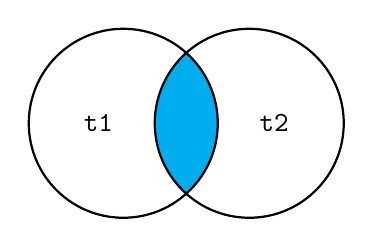
\begin{tikzpicture}[scale=.8]
\begin{scope}
  \clip (0,0) circle(1.5);
  \clip (2,0) circle(1.5);
  \fill[cyan](0,0) circle(1.5cm);
\end{scope}
\draw[thick](0,0)node[left]{\texttt{t1}} circle (1.5);
\draw[thick](2,0)node[right]{\texttt{t2}} circle (1.5);
  \end{tikzpicture}
\end{center}


\begin{lstlisting}
SELECT t1.StockId, t1.Stock, t1.Symbol, t2.Exchange 
    FROM t1 INNER JOIN t2 ON t1.ExchangeId = t2.Id
\end{lstlisting}
\end{frame}


\begin{frame}[fragile]{外联结:左联结}
  左联结(LEFT JOIN)返回左表中的所有行以及右表中满足连接条件的行。
\begin{center}
  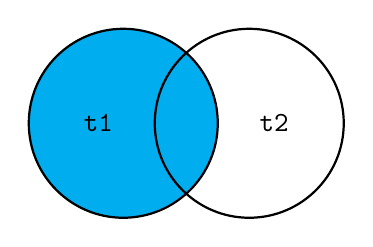
\begin{tikzpicture}[scale=.8]
    \fill[color=cyan](0,0) circle (1.5);
\draw[thick](0,0)node[left]{\texttt{t1}} circle (1.5);
\draw[thick](2,0)node[right]{\texttt{t2}} circle (1.5);
  \end{tikzpicture}
\end{center}
\begin{lstlisting}
SELECT t1.StockId, t1.Stock, t1.Symbol, t2.Exchange 
    FROM t1 LEFT JOIN t2 ON t1.ExchangeId = t2.Id
\end{lstlisting}
\end{frame}


\begin{frame}[fragile]{外联结:右联结}
  右联结(RIGHT JOIN)返回右表中的所有行以及左表中满足连接条件的行。
\begin{center}
  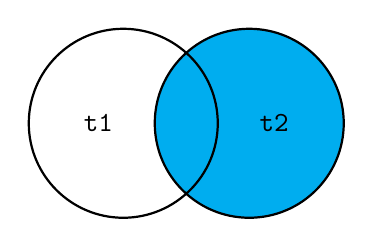
\begin{tikzpicture}[scale=.8]
    \fill[color=cyan](2,0) circle (1.5);
\draw[thick](0,0)node[left]{\texttt{t1}} circle (1.5);
\draw[thick](2,0)node[right]{\texttt{t2}} circle (1.5);
  \end{tikzpicture}
\end{center}
\begin{lstlisting}
SELECT t1.StockId, t1.Stock, t1.Symbol, t2.Exchange 
    FROM t1 RIGHT JOIN t2 ON t1.ExchangeId = t2.Id
\end{lstlisting}
  。
\end{frame}


\begin{frame}[fragile]{外联结:完全联结}
完全联结(FULL JOIN)返回两表中的所有行,无论它们是否匹配

\begin{center}
  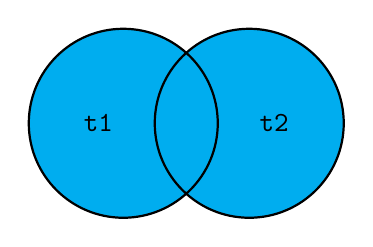
\begin{tikzpicture}[scale=.8]
  \fill[cyan](0,0) circle(1.5);
  \fill[cyan](2,0) circle(1.5);
\draw[thick](0,0)node[left]{\texttt{t1}} circle (1.5);
\draw[thick](2,0)node[right]{\texttt{t2}} circle (1.5);
  \end{tikzpicture}
\end{center}  

在MySQL中,不支持FULL JOIN,所以使用\verb|UNION ALL|运算符来组合\verb|LEFT JOIN|和\verb|RIGHT JOIN|
\end{frame}

\begin{frame}[fragile]{完全联结(cont.)}
  \begin{lstlisting}
    SELECT t1.StockId, t1.Stock, t1.Symbol, t2.Exchange 
        FROM t1 LEFT JOIN t2 ON t1.ExchangeId = t2.Id
      UNION ALL
    SELECT t1.StockId, t1.Stock, t1.Symbol, t2.Exchange 
        FROM t1 RIGHT JOIN t2 ON t1.ExchangeId = t2.Id
    \end{lstlisting}

\begin{block}{注意:}
  使用\verb|UNION ALL|运算符来组合\verb|LEFT JOIN|和\verb|RIGHT JOIN|,进而实现{\color{blue}完全联结}的思路还是存在问题的,会将两个表的{\color{red}内联结部分}重复一次,即:
\[{\color{blue}t_1\cup t_2} + {\color{red}t_1\cap t_2}\]
\end{block}

\end{frame}



\begin{frame}[fragile]{问题所在}
\begin{center}
\begin{tabular}{cccc}
  \hline
  StockId& Stock& Symbol& Exchange\\
  \hline
  2021020100001& 上证指数&000001 &上海证券交易所\\
  2021020100002& 平安银行&000001 &深圳证券交易所\\
  2021020100003 &万科A& 000002 &深圳联合交易所\\
  202000000004 &嘉实增强信用定期债券&000005  \\
  \color{red}2021020100001& \color{red}上证指数&\color{red}000001& \color{red}上海证券交易所\\
  \color{red} 2021020100002 &\color{red}平安银行&\color{red}000001& \color{red}深圳证券交易所\\
  \color{red} 2021020100003 &\color{red}万科A &\color{red}000002& \color{red}深圳联合交易所\\
  &&& 香港联合交易所\\
  \hline
\end{tabular}
\end{center}
\end{frame}


\begin{frame}[fragile]{交叉联结}
  交叉联结(CROSS JOIN)是将左表的每一行与右表的每一行合并。
\begin{center}
\includegraphics[scale=.6]{fig/2-1.jpg}
\end{center}
\begin{lstlisting}
  SELECT t1.StockId, t1.Stock, t1.Symbol, t2.Exchange 
        FROM t1 CROSS JOIN t2 
\end{lstlisting}

\end{frame}

\section{补充内容:使用Python进行联表查询}
\begin{frame}[fragile]{补充内容:使用Python进行联表查询}
基于Python的Pandas包,我们也可以进行联表查询。首先将两个表格转化为DataFrame
\begin{lstlisting}
import pandas as pd
t1 = pd.read_csv('t1.csv', 
                  dtype={'StockId':str, 'Symbol':str})
t2 = pd.read_csv('t2.csv')
\end{lstlisting}

\begin{block}{说明:}
  由于表\verb|t1|当中的\verb|StockId|与\verb|Symbol|都是字符串,为防止Python自动将其视作数值,此处使用字典形式修改这两个字段的类型为字符型(\verb|str|)
\end{block}
\end{frame}

\begin{frame}[fragile]{基于Python的联结}
使用Python进行联表查询,要使用Pandas中的\verb|merge|函数,具体命令如下:
\begin{lstlisting}
df1 = pd.merge(t1, t2, how='inner', left_on='ExchangeId',
                right_on='Id')   # 内联结
df2 = pd.merge(t1, t2, how='left', left_on='ExchangeId',
                right_on='Id')   # 左联结
df3 = pd.merge(t1, t2, how='right', left_on='ExchangeId',
                right_on='Id')   # 右联结
df4 = pd.merge(t1, t2, how='outer', left_on='ExchangeId',
                right_on='Id')   # 完全联结(外联结)
\end{lstlisting}
\end{frame}

\begin{frame}[fragile]{联表查询结果的输出}
以内联结为例,联表查询结果的输出代码如下:
\begin{lstlisting}
print(df1[['StockId', 'Stock', 'Symbol', 'Exchange']])
\end{lstlisting}
这里的输出结果,与SQL语言得到的结果完全相同。

\begin{block}{注意:}
  使用Python进行完全联结所得到的结果,与前面SQL语言得到的结果不同,输出的内容是两个表格的并集,且不存在记录重复的问题。
\end{block}
\end{frame}

\begin{frame}[fragile]{内联结的代码及输出结果}
\begin{lstlisting}
df1 = pd.merge(t1, t2, how='inner', left_on='ExchangeId',
                right_on='Id')   # 内联结
print(df1[['StockId', 'Stock', 'Symbol', 'Exchange']])               
\end{lstlisting}
\begin{center}
  \begin{tabular}{ccccc}
    \hline
   & StockId& Stock & Symbol& Exchange\\
   \hline
    0&  2021020100001&  上证指数 & 000001 & 上海证券交易所\\
    1 & 2021020100002 & 平安银行  &000001&  深圳证券交易所\\
    2  &2021020100003  & 万科A  &000002&  深圳证券交易所\\
    \hline
  \end{tabular}
\end{center}
\end{frame}

\begin{frame}[fragile]{左联结的代码及输出结果}
  \begin{lstlisting}
df2 = pd.merge(t1, t2, how='left', left_on='ExchangeId',
                right_on='Id')   # 左联结
print(df2[['StockId', 'Stock', 'Symbol', 'Exchange']])               
  \end{lstlisting}
  \normalsize
  \begin{center}
    \begin{tabular}{ccccc}
      \hline
     & StockId& Stock & Symbol& Exchange\\
     \hline
      0&  2021020100001&  上证指数 & 000001 & 上海证券交易所\\
      1 & 2021020100002 & 平安银行  &000001&  深圳证券交易所\\
      2  &2021020100003  & 万科A  &000002&  深圳证券交易所\\
      3 &  202000000004 & 嘉实增强信用定期债券 & 000005 &     NaN\\
      \hline
    \end{tabular}
  \end{center}
  \end{frame}

  \begin{frame}[fragile]{右联结的代码及输出结果}
    \begin{lstlisting}
df3 = pd.merge(t1, t2, how='right', left_on='ExchangeId',
                right_on='Id')   # 右联结
print(df3[['StockId', 'Stock', 'Symbol', 'Exchange']])               
    \end{lstlisting}
    \begin{center}
      \begin{tabular}{ccccc}
        \hline
       & StockId& Stock & Symbol& Exchange\\
       \hline
       0 & 2021020100002&  平安银行 & 000001&  深圳证券交易所\\
       1  &2021020100003 &  万科A & 000002 & 深圳证券交易所\\
       2 & 2021020100001  &上证指数&  000001&  上海证券交易所\\
       3  &          NaN   &NaN&     NaN&  香港联合交易所\\
        \hline
      \end{tabular}
    \end{center}
    \end{frame}

  \begin{frame}[fragile]{完全联结的代码及输出结果}
    \begin{lstlisting}
df4 = pd.merge(t1, t2, how='outer', left_on='ExchangeId',
                right_on='Id')   # 完全联结(外联结)
print(df4[['StockId', 'Stock', 'Symbol', 'Exchange']])               
    \end{lstlisting}
    \normalsize
    \begin{center}
      \begin{tabular}{ccccc}
        \hline
       & StockId& Stock & Symbol& Exchange\\
       \hline
      0&  2021020100001&  上证指数 & 000001 & 上海证券交易所\\
      1 & 2021020100002 & 平安银行  &000001&  深圳证券交易所\\
      2  &2021020100003  & 万科A  &000002&  深圳证券交易所\\
      3 &  202000000004 & 嘉实增强信用定期债券 & 000005 &     NaN\\
      4 &          NaN   &NaN&     NaN&  香港联合交易所\\
        \hline
      \end{tabular}
    \end{center}
    \end{frame}










\end{document}

